\section{Patrones de Diseño}
	\noindent Los patrones de diseño permiten organizar el código de forma flexible, reutilizable y mantenible. A continuación se describen los patrones más relevantes que se aplicarán al sistema \textbf{Casa Fácil}:
	
	\subsection*{1. Strategy Pattern}
		\noindent Este patrón permite definir diferentes algoritmos para una misma tarea y cambiarlos dinámicamente según la necesidad, manteniendo la misma interfaz.  
		\textbf{Aplicación:} En la búsqueda de inmuebles, se pueden aplicar múltiples estrategias: por precio, por cercanía a una universidad o por reglas del inmueble (como "no fumar", "sin mascotas"), sin modificar la lógica principal del buscador.
		\begin{center}
			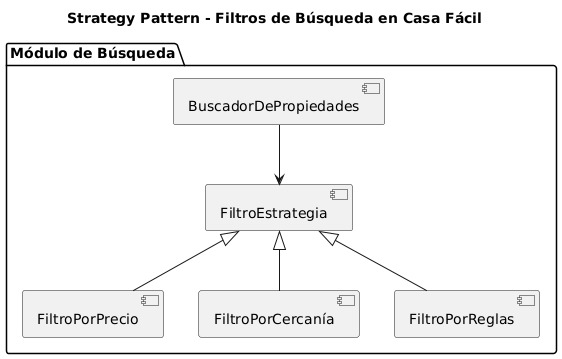
\includegraphics[width=\linewidth]{figures/patterns/strategy.jpg}
			\captionof{figure}{Patron de diseño Strategy.}
			\label{fig:img9}
		\end{center}
	
	\subsection*{2. Observer Pattern}
		\noindent Define una relación de dependencia uno-a-muchos, de modo que cuando un objeto cambia de estado, todos los observadores reciben notificaciones automáticamente.  
		\textbf{Aplicación:} Los usuarios que se suscriban a una propiedad recibirán notificaciones automáticas cuando cambie su disponibilidad o precio.
		\begin{center}
			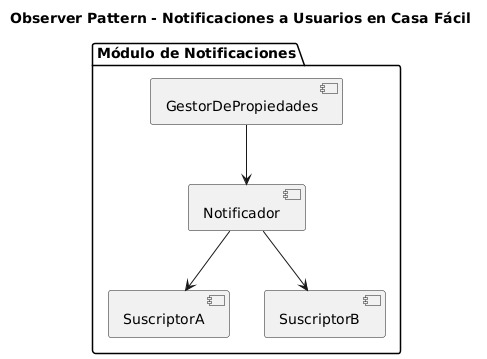
\includegraphics[width=\linewidth]{figures/patterns/observe.jpg}
			\captionof{figure}{Patrón de diseño Observer.}
			\label{fig:img10}
		\end{center}
	
	\subsection*{3. Facade Pattern}
		\noindent Proporciona una interfaz unificada y simplificada a un conjunto de funcionalidades complejas.  
		\textbf{Aplicación:} Puede encapsular toda la lógica de reservas, pagos o validaciones en una clase fachada, de modo que el frontend interactúe con un solo punto de entrada, simplificando las integraciones.
		\begin{center}
			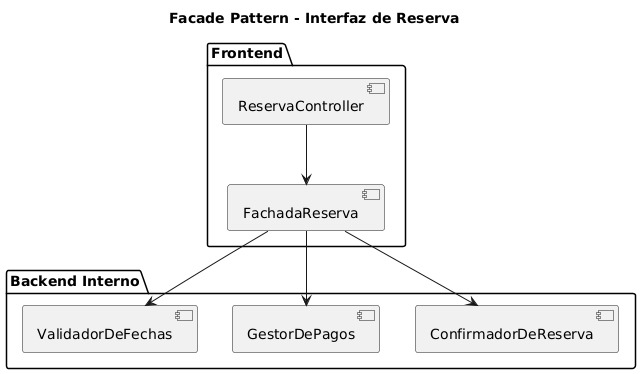
\includegraphics[width=\linewidth]{figures/patterns/facade.jpg}
			\captionof{figure}{Patrón de diseño Facade.}
			\label{fig:img11}
		\end{center}
	
	\subsection*{4. Decorator Pattern}
		\noindent Permite extender dinámicamente el comportamiento de un objeto envolviéndolo con nuevos componentes, sin modificar su clase original.  
		\textbf{Aplicación:} El sistema de notificaciones puede comenzar con envíos por correo electrónico, y luego extenderse fácilmente a SMS o WhatsApp mediante decoradores.
		\begin{center}
			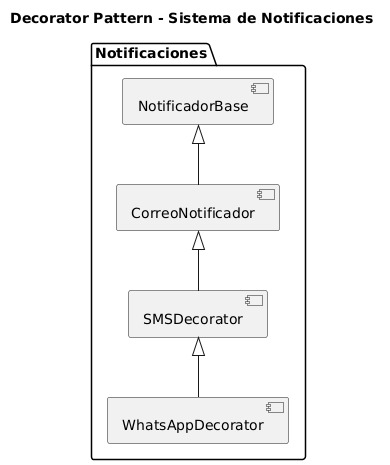
\includegraphics[width=\linewidth]{figures/patterns/decorator.jpg}
			\captionof{figure}{Patrón de diseño Decorator.}
			\label{fig:img12}
		\end{center}
	
	\subsection*{5. Singleton Pattern}
		\noindent Garantiza que una clase tenga una única instancia durante todo el ciclo de vida del sistema, y proporciona un acceso global a ella.  
		\textbf{Aplicación:} Puede utilizarse para gestionar una única instancia del sistema de configuración o autenticación del sistema.
		\begin{center}
			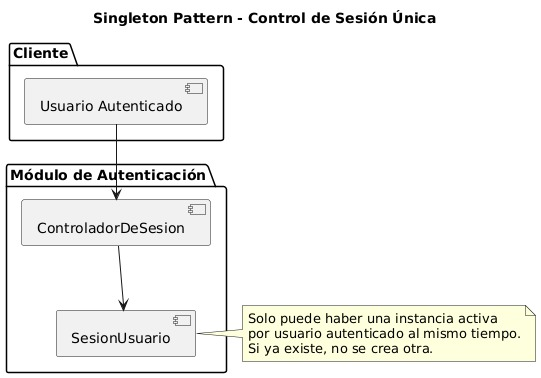
\includegraphics[width=\linewidth]{figures/patterns/singleton.jpg}
			\captionof{figure}{Patrón de diseño Singleton.}
			\label{fig:img13}
		\end{center}
	
	\subsection*{6. Factory Pattern}
		\noindent Permite crear objetos sin exponer su lógica de creación al cliente, utilizando una interfaz común.  
		\textbf{Aplicación:} Se puede usar para crear diferentes tipos de usuarios (inquilino, propietario, administrador), propiedades o métodos de pago, desde una misma factoría base.
		\begin{center}
			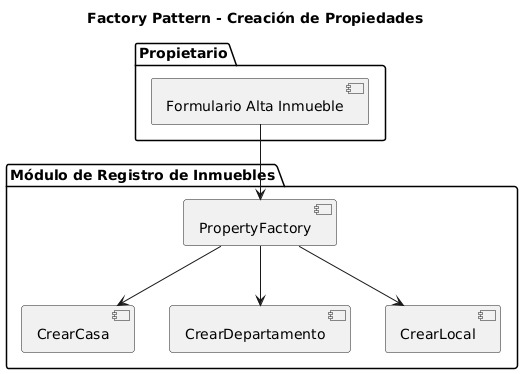
\includegraphics[width=\linewidth]{figures/patterns/factory.jpg}
			\captionof{figure}{Patrón de diseño Factory.}
			\label{fig:img14}
		\end{center}
	
	\subsection*{7. Repository Pattern}
		\noindent Actúa como una capa intermedia entre la lógica de negocio y la base de datos, permitiendo un acceso estructurado y mantenible.  
		\textbf{Aplicación:} Se puede aplicar para generar repositorios reutilizables de entidades como propiedades, usuarios o mensajes.
		\begin{center}
			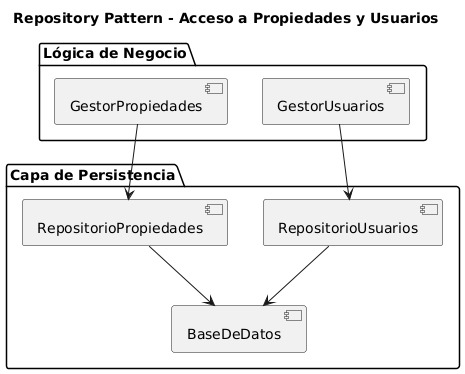
\includegraphics[width=\linewidth]{figures/patterns/repository.jpg}
			\captionof{figure}{Patrón de diseño Repository.}
			\label{fig:img15}
		\end{center}
	
	\subsection*{8. Composite Pattern}
		\noindent Permite tratar objetos individuales y estructuras jerárquicas de manera uniforme.  
		\textbf{Aplicación:} Es útil para representar jerarquías de reglas (por ejemplo, reglas generales y subreglas por inmueble), o categorías y subcategorías de propiedades (como “Habitaciones” → “Amuebladas” / “Sin amueblar”).
		\begin{center}
			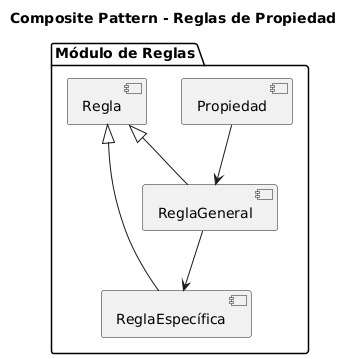
\includegraphics[width=\linewidth]{figures/patterns/composite.jpg}
			\captionof{figure}{Patrón de diseño Composite.}
			\label{fig:img16}
		\end{center}
		
	\subsection*{9. Lazy Loading}
		\noindent Retrasa la carga de recursos hasta que realmente se necesitan.  
		\textbf{Aplicación:} Imágenes, videos, mapas o reseñas de propiedades pueden cargarse solo cuando el usuario interactúe con ellos, mejorando así el rendimiento general del sistema.
		\begin{center}
			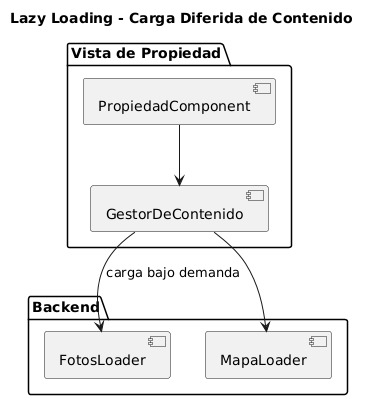
\includegraphics[width=\linewidth]{figures/patterns/lazy.jpg}
			\captionof{figure}{Patrón de diseño Lazy Loading.}
			\label{fig:img17}
		\end{center}
		
	\newpage
	\subsection*{10. Principios SOLID}
		\noindent Los principios SOLID permiten crear software más mantenible, modular y fácil de probar. Son esenciales al trabajar con microservicios y arquitecturas escalables como la de \textbf{Casa Fácil}.
		
		\begin{itemize}
			\item \textbf{S - Single Responsibility Principle:} Cada clase debe tener una única responsabilidad. En Casa Fácil, por ejemplo, un servicio dedicado solo a manejar pagos o reservas.
			
			\item \textbf{O - Open/Closed Principle:} El código debe estar abierto a extensión, pero cerrado a modificación. Por ejemplo, al agregar nuevas formas de pago sin alterar el código original, se puede usar el patrón Strategy.
			
			\item \textbf{L - Liskov Substitution Principle:} Las clases derivadas deben poder sustituir a sus clases base sin afectar el funcionamiento. Por ejemplo, una clase \texttt{UsuarioPremium} debe poder sustituir a \texttt{Usuario} sin romper la lógica.
			
			\item \textbf{I - Interface Segregation Principle:} Es mejor tener interfaces pequeñas y específicas que una general demasiado extensa. Un controlador de publicaciones no debería forzarse a implementar métodos de notificación si no los necesita.
			
			\item \textbf{D - Dependency Inversion Principle:} Las clases deben depender de abstracciones, no de clases concretas. Esto permite inyectar servicios como repositorios o validadores sin acoplarlos al código del controlador.
		\end{itemize}